% Zapallitos Italianos Rellenos
\newpage
%\thispagestyle{empty}
\begin{recipe}[source={La Mami y Youtube},
portion={6 porciones},
preparationtime={\unit[1]{Hora}}
]{Zapallitos Italianos Rellenos}
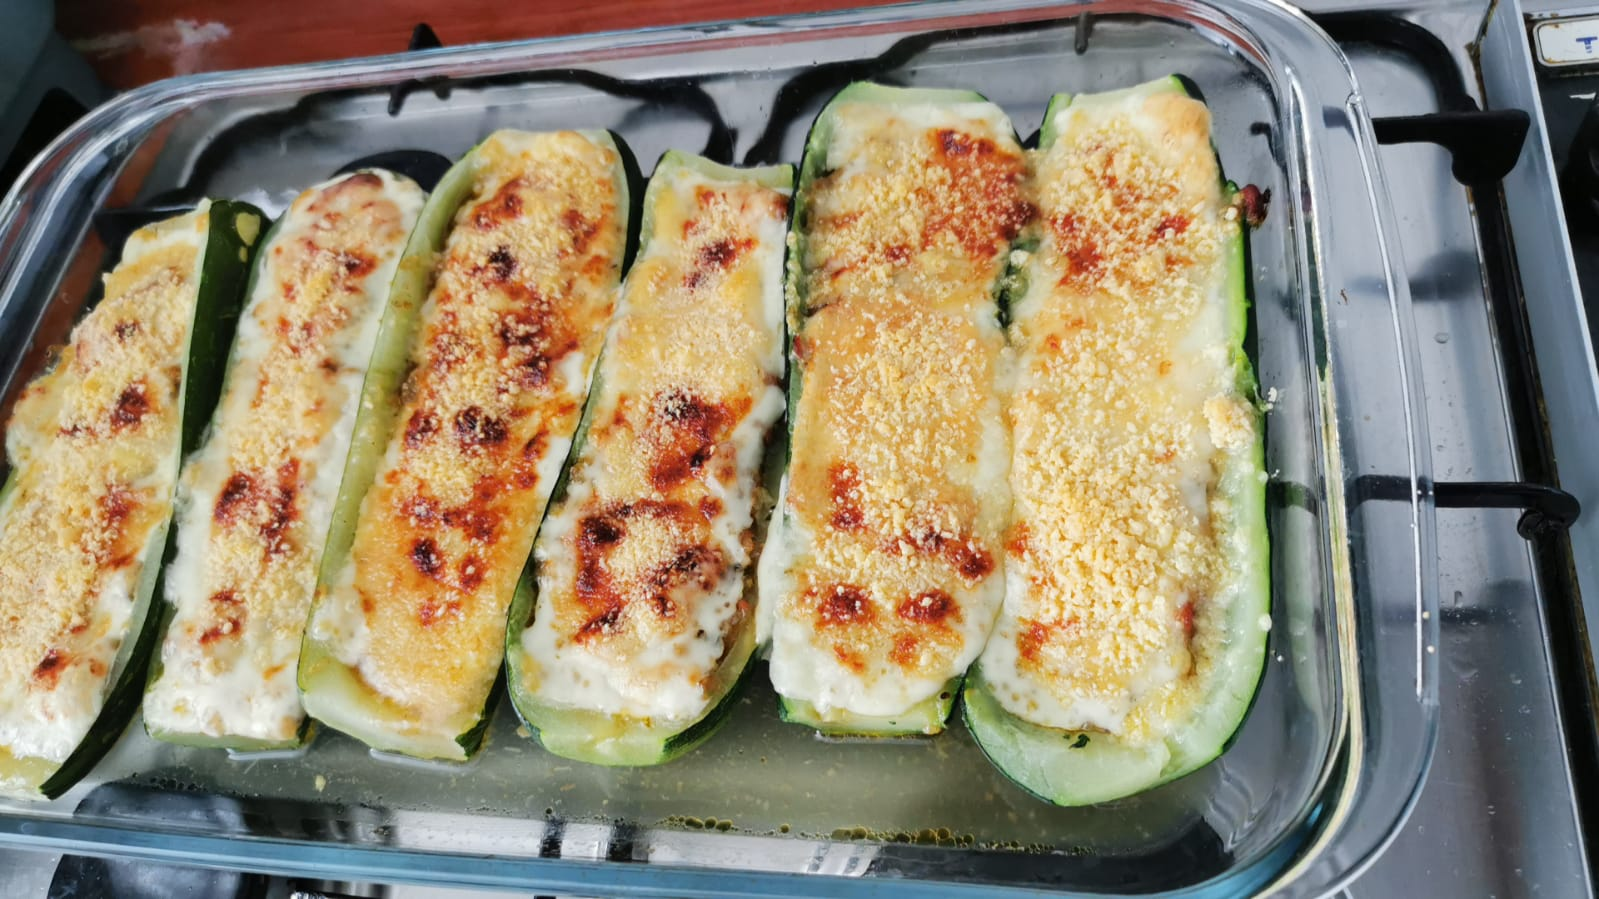
\includegraphics[width=0.25\textwidth]{zapallos-italianos}
	\introduction{
		Los zapallos italianos son una receta típica de la familia. Son muy ricos para comer solos, o acompañándolos con algún arroz o ensalada.
	}
	\ingredients{
		\unit[250]{gr} & posta molida de vacuno o cualquier corte magro \\
		3 & zapallos Italianos \\
		2 & cucharadas de aceite de oliva \\
		1 & taza de cebolla picada finamente en cuadraditos \\
		3 & dientes de ajo \\
		1 & cucharada de paprika o ají de color \\
		1 & cucharada de orégano fresco \\
		& Sal a gusto \\
		& Queso rallado
	}
	\preparation{
		\begin{enumerate}
			\item Cortar los zapallos italianos a lo largo a la mitad.
			\item Rascar los zapallos italianos por dentro de tal manera de ir dejando una
			      especie de canal por dentro y extraer el centro. Para esto se puede valer de
			      una cuchara.
			\item Cocer las mitades ya partidas y rascadas 10 minutos en agua hirviendo con sal.
			\item Para el relleno, en una olla se prepara un sofrito echando un poco del aceite
			      con el ajo picándolo finamente y agregando la cebolla, el orégano y finalmente
			      el relleno extraído de los zapallos, un poco de sal y revolviendo a fuego suave
			      entre 15 y 20 minutos.
			\item Escurrir los zapallos y extraer el relleno y colocar en una fuente para horno.
			\item Precalentar el horno a 180 grados con calor arriba y abajo durante 5 minutos.
			\item En la fuente colocar los zapallos y rellenar con el relleno preparado,
			      posteriormente decorar con el queso rallado y meter la fuente al horno hasta
			      que el queso quede gratinado por aproximadamente 15 minutos.
			\item retirar del horno y servir.
		\end{enumerate}
	}
\end{recipe}